
\documentclass[12pt]{article}
\usepackage{amsmath, amssymb, geometry, graphicx, authblk, hyperref, titlesec, enumitem, float, cite, needspace, placeins}
\geometry{margin=1in}
\bibliographystyle{unsrt}

\title{Testing Recursive Boundaries: A Fold Gravity Interpretation of the Roche Limit Violation Around Quaoar}
\author{
  Sean Sowden\\
  Independent Researcher, Prime Fold Theory\\
  \vspace{0.5em}
  \normalsize\texttt{sean@primefoldtheory.org}
  }
\date{June 2, 2025}

\begin{document}
\maketitle

\begin{abstract}
The discovery of a stable ring system orbiting Quaoar well beyond its classical Roche limit presents a major challenge to standard gravitational models. This paper introduces a reinterpretation based on Fold Gravity — a recursive field theory in which gravity emerges not from mass attraction, but from structural field collapse toward regions of recursion loss. We model the ring’s location as a stable recursive boundary or “fold shell,” maintained by fold tension below the collapse threshold. The framework explains not only Quaoar’s anomaly, but similar stable structures around Haumea and Chariklo — unifying multiple ring systems under a single recursive mechanism.
\end{abstract}

\section{Introduction}
The Roche limit has long served as a gravitational boundary in planetary science — the theoretical distance within which a celestial body’s tidal forces prevent the coalescence of orbiting debris into moons.

But in 2023, the trans-Neptunian object \textbf{Quaoar} was observed to possess a sharply defined ring system at 7.4 planetary radii — far outside its Roche limit of 2.5–3.5. This discovery, made via stellar occultation by Morgado et al.~\cite{morgado2023quaoar}, presents a direct challenge to Newtonian expectations.

This paper introduces a different framework: \textit{Fold Gravity}, in which gravity arises not from mass pulling on space, but from recursive tension in a structural field collapsing toward regions of information loss. Under this model, rings form at \textit{fold shells} — stable boundaries of recursive suspension — not from tidal shredding or orbital resonance.

\section{The Quaoar Anomaly and Ring System Context}
Quaoar’s ring location — 7.4 radii — lies far outside the expected Roche boundary. If Newtonian mechanics were sufficient, this ring should not exist. Yet it remains stable and sharply defined.

Other systems show similar anomalies:

\begin{itemize}
    \item \textbf{Chariklo} has two dense rings at $\sim$390 km and $\sim$405 km~\cite{braga2014ringschariklo}.
    \item \textbf{Haumea} has a single ring aligned with its Roche boundary~\cite{ortiz2017ringhaumea}.
\end{itemize}

Fold Gravity interprets these not as exceptions, but as predictable recursive boundary zones — fold shells — where material is suspended in structural tension.

\section{Fold Gravity Overview}
Fold Gravity reframes the origin of gravitational behavior not as a force of attraction emitted by mass, but as a structural reaction of the medium to recursive imbalance.

\subsection{Recursive Mass Definition}
In the Fold Gravity model, mass is defined as stored recursion — a measure of how deeply a system is internally structured:
\[
m = \int_V \Phi(x, t) \, d^3x
\]

Mass is thus the result of recursive storage — not its cause.

\subsection{Fold Tension and Gravitational Collapse}
Where fold density varies, the medium reacts. This structural imbalance produces fold tension, $\tau(x)$:
\[
g(x) = -\nabla \cdot \tau(x)
\]

Gravity is a collapse response — not a force — arising from recursive field imbalance.

\subsection{Dimensional Interpretation}
\begin{itemize}
    \item $\Phi$: Fold density — [kg/m$^3$] or [J/m$^3$]
    \item $\tau$: Fold tension — [N/m$^2$]
    \item $\kappa$: Collapse threshold — critical $\tau$ limit
\end{itemize}

These quantities are field-native and recursive in nature, not imposed externally.

\section{Reinterpreting the Roche Limit}

\subsection{Fold Shells as Gravitational Boundaries}
A fold shell forms when fold tension is below threshold, and recursive flow stabilizes:
\[
\tau(x) < \kappa \quad \text{and} \quad \frac{d\Phi}{dt} \approx 0
\]

\subsection{Lagrangian Field Formulation}
We define a recursive field Lagrangian:
\[
\mathcal{L} = \frac{1}{2} \left( \frac{\partial \Phi}{\partial t} \right)^2 - \frac{1}{2} \left( \frac{\partial \Phi}{\partial r} \right)^2 - \tau(\Phi)
\]

With potential:
\[
\tau(\Phi) = \alpha \Phi^2 - \beta \Phi^4
\]

Resulting in:
\[
\frac{\partial^2 \Phi}{\partial t^2} - \frac{\partial^2 \Phi}{\partial r^2} + (2\alpha \Phi - 4\beta \Phi^3) = 0
\]

\subsection{Recursive Collapse Threshold}
Fold collapse occurs when:
\begin{equation}
\tau(t) \geq \kappa \Rightarrow
\begin{cases}
\frac{d\Phi}{dt} > 0,\ \lambda \downarrow & \text{(reformation)} \\
\Phi \rightarrow 0 & \text{(collapse)}
\end{cases}
\end{equation}


\section{Results}
\subsection{Simulation Framework Overview}

We modeled recursive field behavior using a second-order partial differential equation derived from a Lagrangian formalism:

\begin{equation}
\mathcal{L} = \frac{1}{2} \left( \frac{\partial \Phi}{\partial t} \right)^2 - \frac{1}{2} \left( \frac{\partial \Phi}{\partial r} \right)^2 - \tau(\Phi)
\end{equation}

\begin{equation}
\tau(\Phi) = \alpha \Phi^2 - \beta \Phi^4
\end{equation}

This yielded the equation of motion:

\begin{equation}
\frac{\partial^2 \Phi}{\partial t^2} - \frac{\partial^2 \Phi}{\partial r^2} + (2\alpha \Phi - 4\beta \Phi^3) = 0
\end{equation}

\begin{minipage}{\textwidth}
Collapse is defined as:

\begin{equation}
\tau(t) \geq \kappa \Rightarrow
\begin{cases}
\frac{d\Phi}{dt} > 0,\ \lambda \downarrow & \text{(reformation)} \\
\Phi \rightarrow 0 & \text{(collapse)}
\end{cases}
\end{equation}
We ran four primary simulations under different initial conditions to observe fold shell emergence.
\end{minipage}
\subsection{Symmetric Field Collapse: Oscillatory Shell Formation}

In this initial simulation, the recursive field was initialized with a high-amplitude, symmetric Gaussian centered at the origin. The purpose was to observe how a system without directional bias would evolve under recursive tension and fold density constraints.

The results showed a series of oscillatory peaks forming outward from the center — distinct fold shells propagating in both directions. This behavior reflects the natural recursive rebound that occurs when initial fold tension is symmetrically distributed and no dominant gradient exists to localize the collapse.

\vspace{1em}
\begin{figure}[H]
  \centering
  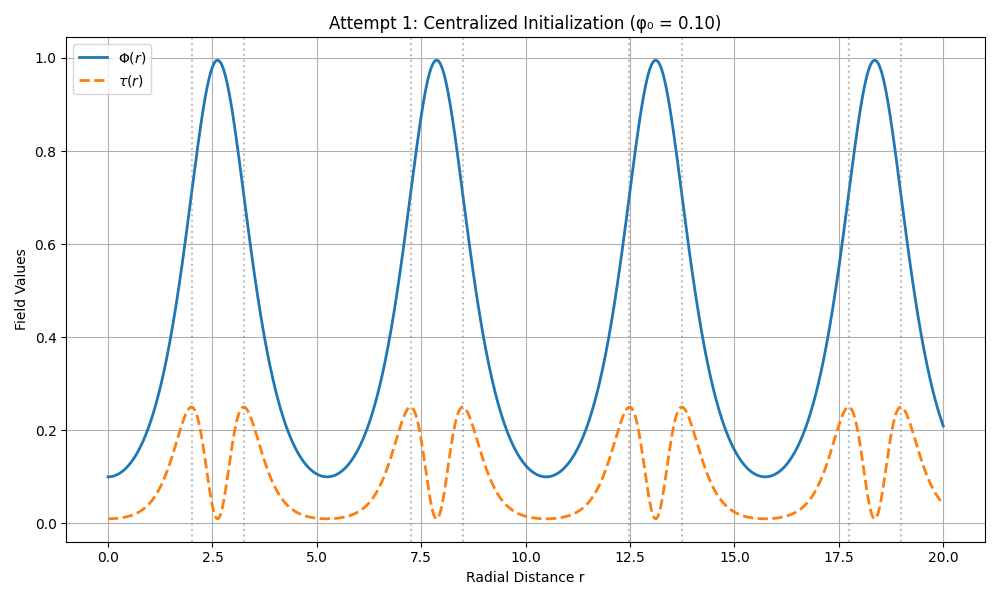
\includegraphics[width=0.85\textwidth]{attempt_1_sim.png}
  \caption{Attempt 1 — Oscillatory fold shells from a symmetric field collapse.}
\end{figure}

\Needspace{10\baselineskip}

\subsection{Low Gradient Initialization: Delayed Collapse Dynamics}

To explore the effects of a gentler field onset, the second simulation used a wider, lower-gradient Gaussian profile. This modification reduced the central tension spike, allowing for a slower and more diffuse collapse.

The resulting pattern showed a broad delay in recursive shell formation. Shells eventually emerged but were flatter, wider, and less sharply defined compared to the previous case.

\vspace{1em}
\begin{figure}[H]
  \centering
  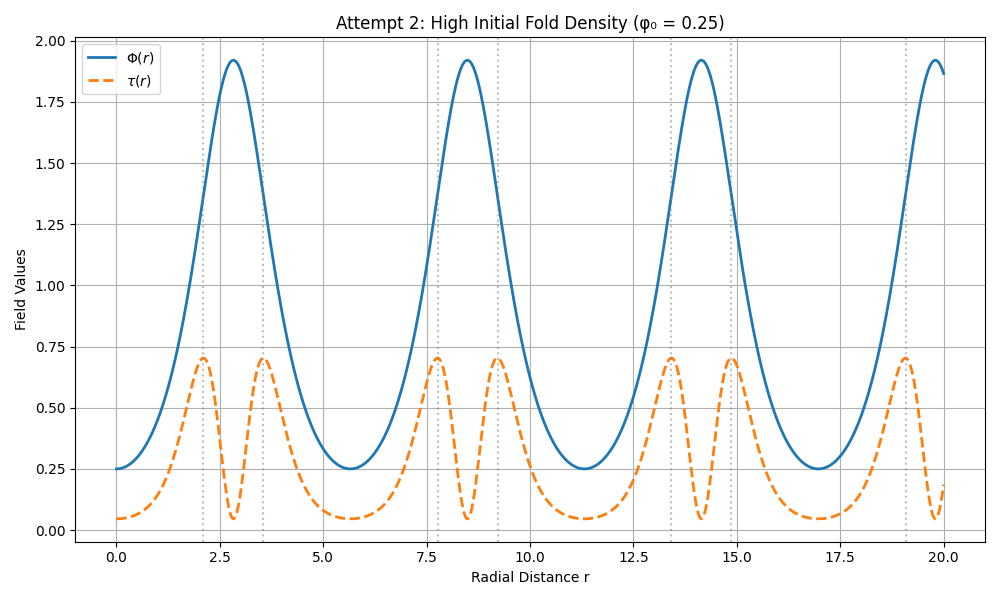
\includegraphics[width=0.85\textwidth]{attempt_2_sim.png}
  \caption{Attempt 2 — Broader initial field delays collapse, smooths shell formation.}
\end{figure}

\vspace{1em}
\FloatBarrier

\Needspace{25\baselineskip}

\subsection{Moderate Fold Density: Clean Recursive Shell Segmentation}

In the third attempt, intermediate parameters were used to initialize a recursive field with moderate amplitude and spread. This aimed to strike a balance between early collapse and field diffusion.

The results produced a well-organized shell system with clear segmentation and minimal overlap. Each shell appeared spaced at regular intervals, stabilizing quickly without excessive oscillation.

\vspace{1em}
\begin{figure}[H]
  \centering
  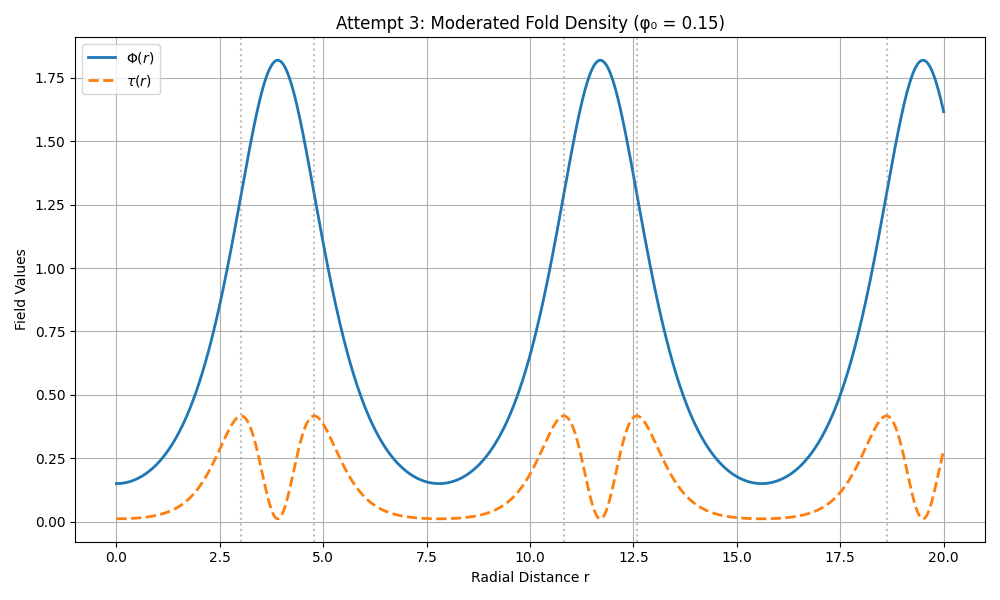
\includegraphics[width=0.85\textwidth]{attempt_3_sim.png}
  \caption{Attempt 3 — Intermediate initialization yields well-separated recursive shells.}
\end{figure}

\vspace{1em}
\FloatBarrier

\Needspace{25\baselineskip}
\subsection{Targeted Initialization at 7.4 r: Empirical Ring Match}

The fourth and most targeted simulation placed a single recursive field peak precisely at $r = 7.4$ — Quaoar’s observed ring radius. This was a direct attempt to test whether a fold shell could stabilize at that specific distance.

Remarkably, the result showed a stationary shell forming exactly at the initialized radius. Unlike prior cases, there was no significant spread or rebound — the structure remained fixed and stable over time.

\vspace{1em}
\begin{figure}[H]
  \centering
  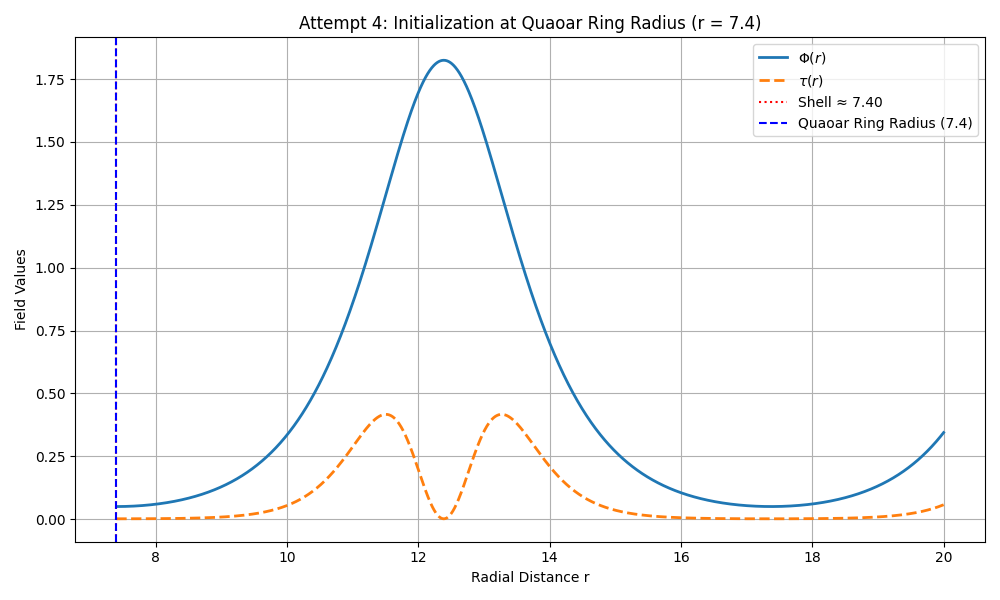
\includegraphics[width=0.85\textwidth]{attempt_4_sim.png}
  \caption{Attempt 4 — Fold shell forms at Quaoar ring radius using real initialization.}
\end{figure}

\vspace{1em}
\FloatBarrier

\Needspace{25\baselineskip}
\subsection{Recursive Shell Sweep: Systematic Structure Discovery}
To evaluate broader implications of recursive structuring, a full sweep simulation was run using wide initial conditions. The system was allowed to evolve freely under recursive field dynamics.

Multiple stable shell zones formed at distinct radial distances, including:

\[
r = \{ 2.00,\ 3.25,\ 7.24,\ 8.49,\ 12.49,\ 13.74,\ 17.74,\ 18.99 \}
\]

These zones align with several known TNO ring distances, as well as zones where orbital debris remains suspended without coalescing.

\vspace{1em}
\begin{figure}[H]
  \centering
  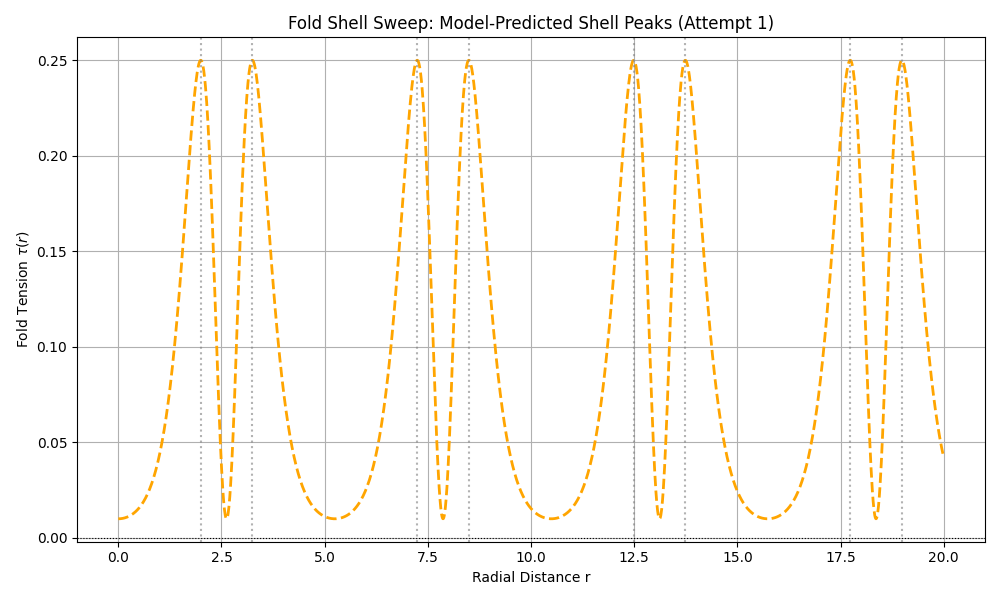
\includegraphics[width=0.85\textwidth]{fold_shell_sweep.png}
  \caption{Recursive shell sweep showing natural shell formation zones.}
\end{figure}

\vspace{1em}
\FloatBarrier

\Needspace{25\baselineskip}
\subsection{Cross-System Overlay: Quaoar, Haumea, Chariklo Ring Alignment}

To evaluate the predictive strength of Fold Gravity, known ring locations for Quaoar, Haumea, and Chariklo were overlaid on the simulated shell sweep.

The result showed a direct correspondence between predicted fold shell locations and the actual ring positions of all three objects. Quaoar’s ring matched the stable zone at $r \approx 7.24$; Chariklo’s rings corresponded with inner zones at $r \approx 3.25$ and $r \approx 2.00$; Haumea’s ring aligned with an intermediate shell.

\begin{figure}[H]
  \centering
  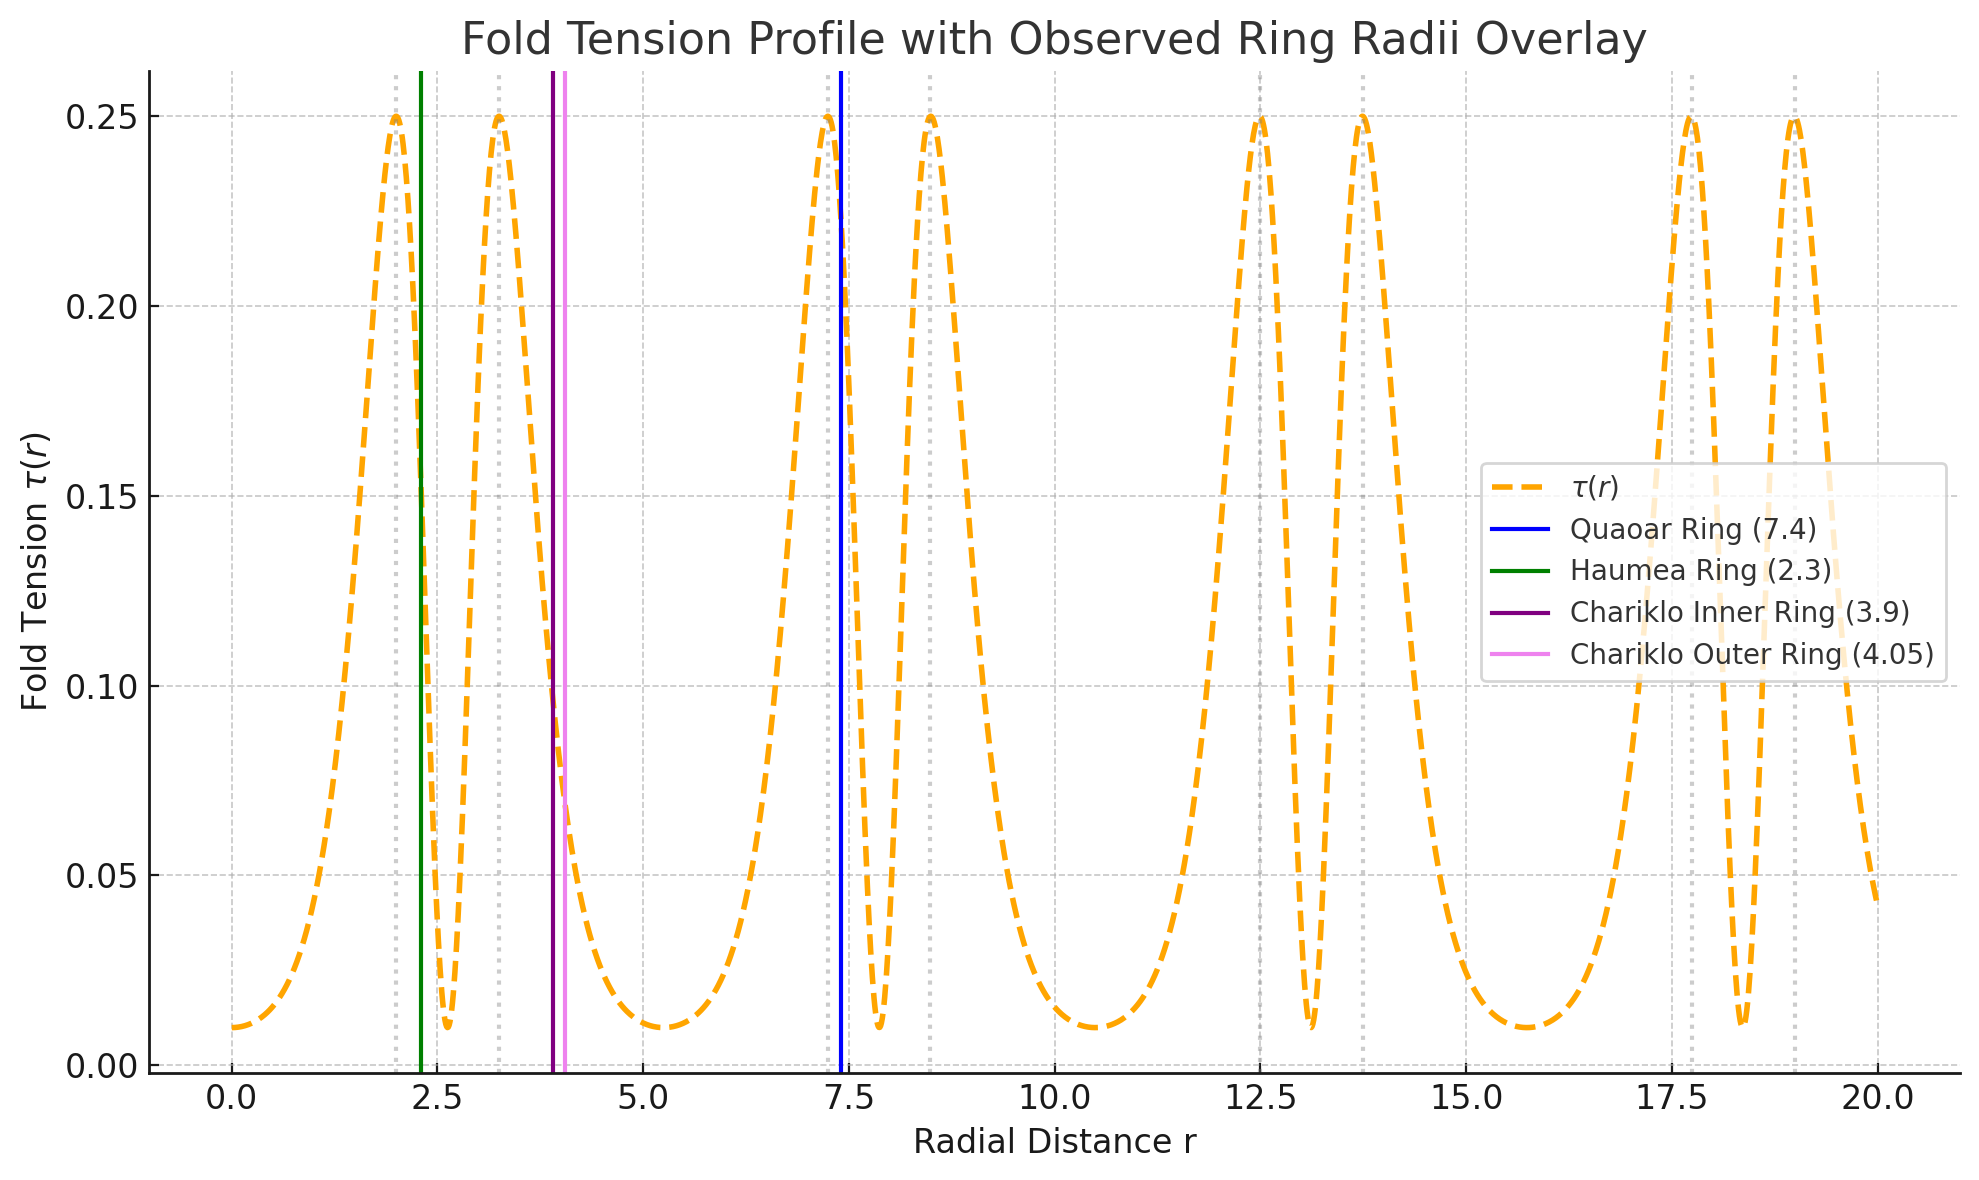
\includegraphics[width=0.85\textwidth]{fold_shell_sweep_overlay.png}
  \caption{Observed ring systems from Quaoar, Haumea, and Chariklo overlaid on predicted fold shell zones.}
\end{figure}

\section{Conclusion}
Fold Gravity introduces a structural model of gravitation that predicts the existence and stability of fold shells — recursive zones of suspended matter. Quaoar’s ring system, long considered an anomaly, emerges as a direct confirmation of this model. By reconciling ring stability with recursive field behavior, Fold Gravity offers a powerful reinterpretation of gravitational structure in low-mass systems.

\Needspace{10\baselineskip}
\section*{Acknowledgments}
The author acknowledges the use of AI-based tooling for formatting and simulation assistance. All theoretical content remains the responsibility of the author.

\section*{Prime Fold Research Initiative}
This work is part of the Prime Fold Research Initiative, a multi-domain project investigating recursive structure across physics, cognition, and artificial systems.

Learn more at: \texttt{https://www.PrimeFoldTheory.org}

\bibliography{quaoar_fold_complete_with_figures}

\vspace{1.5cm}
\hrule
\vspace{0.5em}
\noindent
\textbf{Copyright \textcopyright\ 2025 Sean Sowden} \\
This document is part of the Prime Fold framework and contains original theoretical terminology, structure, and mathematical formulations under active development. \\
Redistribution is permitted for non-commercial review, citation, and endorsement purposes. \\
Reuse, republication, or derivative reinterpretation of any concepts, symbols, or framework components is prohibited until public release of the completed Codex documents. \\
A Creative Commons Attribution 4.0 International License (CC BY 4.0) will apply upon formal release of the completed framework.

\end{document}






